\section{Die Algorithmen auf diesem Markt}
Der Vergleich der RL-Algorithmen findet auf dem in \ref{section:markov} definierten Markt statt.
Dieser Markt wird auf der Testplattform simuliert, die im Rahmen des Bachelorprojektes entwickelt wurde.
Er wird über die Gym-Schnittstelle durch die Agenten angesprochen.
Für die zu vergleichenden Algorithmen werden hauptsächlich die Implementierungen der Bibliothek \textit{Stable Baselines} verwendet. \cite{stable-baselines}
Stable Baselines ist eine weit verbreitete eine Open-Source RL-Bibliothek, die in Python geschrieben ist.
Sie baut auf PyTorch auf, einem der beliebtesten Deep-Learning-Frameworks, das in der Forschung weite Verbreitung findet. \cite{NEURIPS2019_9015}
Die in Stable Baselines implementierten Algorithmen entsprechen in den meisten Fällen unmittelbar den vorgeschlagenen Algorithmen der Originalpaper und zeichnen sich durch eine hohe Lesbarkeit des Codes aus.
Alle Hyperparameter sind konfigurierbar.

In dieser Untersuchung der Algorithmen wird stets von den Hyperparametern der Originalpaper ausgegangen.
Weil kaum theoretische Erkenntnisse über die Ermittlung optimaler Hyperparameter vorliegen und diese stets problemspezifisch sind, ist eine erschöpfende Optimierung der Hyperparameter nur mit erheblichem experimentellem Aufwand möglich.
Dazu müssten sehr viele Kombinationen mit jeweils mehreren Läufen durchgeführt werden, was einen nicht zu leistenden Ressourcenaufwand darstellt.
Dennoch wurden an einigen Stellen bessere Hyperparameter gefunden und Aussagen über die Algorithmen über mehrere Hyperparameterkombinationen abgesichert.

Alle Verfahren werden mit neuronalen Netzen durchgeführt, die zwei versteckte Schichten mit je 64 Neuronen haben.
Das Verhalten der Algorithmen für unterschiedliche Netzgrößen ist aber sehr ähnlich, wie die Experimente mit unterschiedlichen Netzgrößen im Bereich [noch zu erstellen] des Anhangs zeigen.
Für den Vergleich der Algorithmen werden diese zunächst innerhalb ihrer Gruppen betrachtet und auf generelle Eignung für dieses Setup geprüft.
Danach werden die Algorithmen, die sich als grundsätzlich geeignet erwiesen haben, hinsichtlich verschiedener Kriterien verglichen.
Alle Messungen wurden auf dem Duopol-Szenario durchgeführt.

\section{DDPG und TD3}
\label{section:main_ddpg}
Bei der Diskussion der Q-Learning-Verfahren beschränkt sich diese Analyse direkt auf die Verfahren, die im stetigen Raum angewendet werden.
Deep-Q-Networks mit diskreten Aktionen müssen jede einelne Aktion aus $\mathcal{A_\mathbb{N}}$ mit einem Aktionswert versehen.
Das sind bei der Konfiguration mit $p_{max}=10$ bereits 1000 Ausgabeneuronen und das Wachstumsverhalten ist kubisch in der Anzahl der Preisstufen.
Diese Eigenschaft verhindert den Einsatz für DQNs und Verfahren mit diskreten Aktionsräumen allgemein für dieses Problem.
Im Anhang zeigt Diagramm [noch zu erstellen] das Training von DQNs auf diesem Setup und bestätigt dessen Untauglichkeit.

\begin{figure}[htbp]
	\centering
	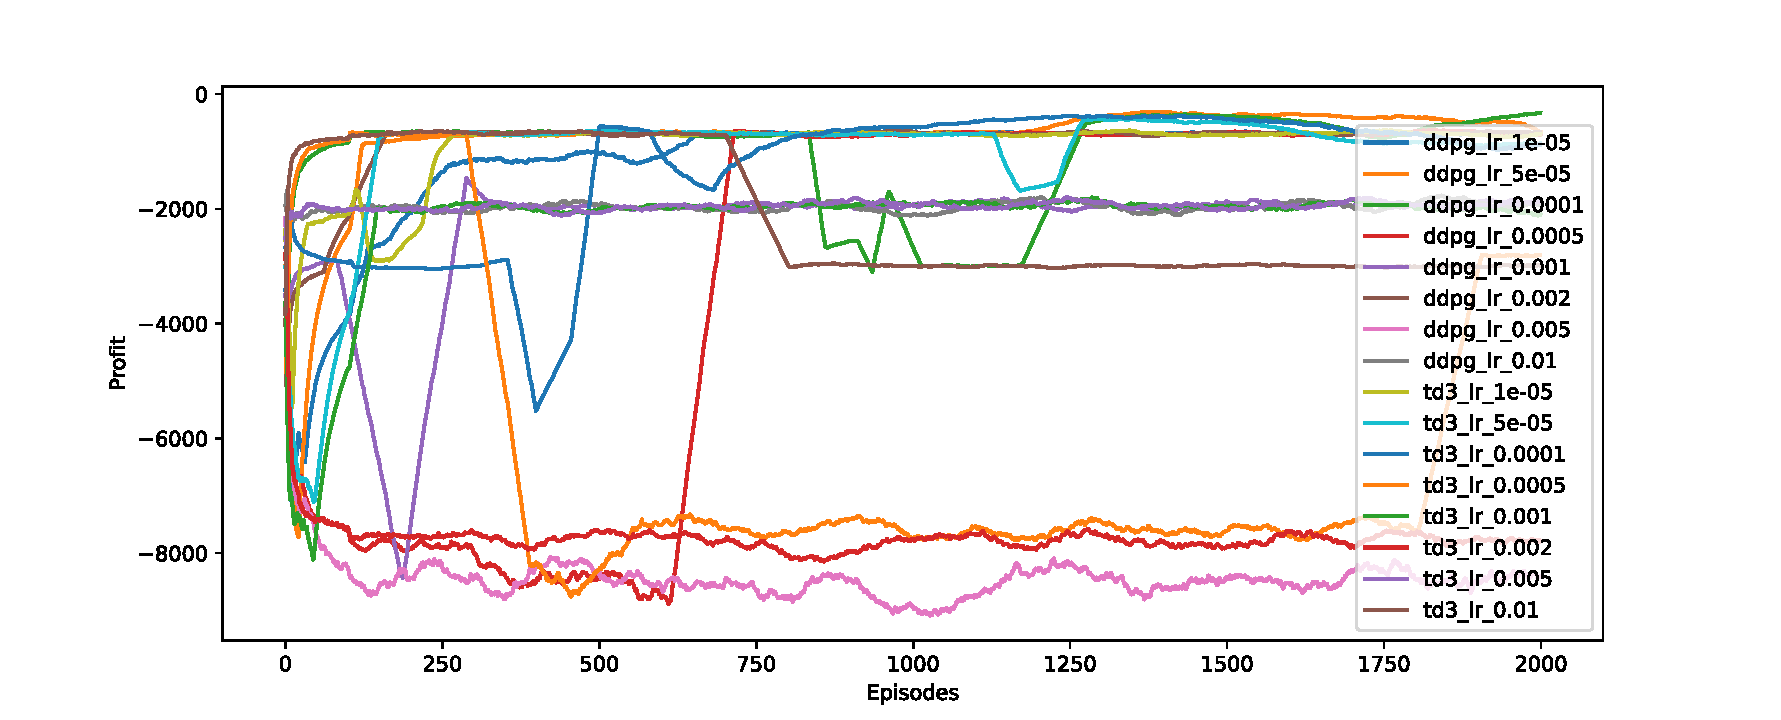
\includegraphics[width=\textwidth]{main/DDPG_learning_curve.pdf}
	\caption{Lernkurven von DDPG und TD3 mit unterschiedlichen Lernraten}
	\label{grafic:DDPGLearningCurve}
\end{figure}

Die Lernkurven der beiden sehr ähnlichen Verfahren DDPG und TD3 sind in Abbildung \ref{grafic:DDPGLearningCurve} dargestellt.
Für jeden der beiden Algorithmen wurden acht Trainingsläufe durchgeführt, die mit unterschiedlichen Lernraten parametrisiert wurden.
Der Standardwert liegt für beide Algorithmen bei $1e-3$.
Es wurden Trainingsläufe mit diesen Lernraten sowie kleineren und größeren durchgeführt.
Die beim Training beobachteten Muster gleichen sich sowohl bei den beiden Algorithmen als auch den unterschiedlichen Parametrisierungen.

Zu Beginn des Trainings ist bei einigen Läufen eine Verbesserung der gemittelten Returns, die primäre Leistungskennziffer, zu beobachten.
Allerdings kommt diese Verbesserung bei allen Algorithmen zum Erliegen und eine konstante Leistung stellt sich ein.
Dabei treten Häufungen bei der Leistung -2000 und -700 auf.
Bei einigen Trainingsdurchläufen wird ein Niveau von -300 erreicht, dieses aber nie überschritten.

Betrachtet man die Zusammensetzung der Gewinne -- die Diagramme dazu befinden sich im Anhang -- erkennt man, dass ein Teil der Agenten durch das Setzen hoher Neupreise wenige Kunden mit hoher Rendite gewinnen konnte.
Die mit dem Neuverkauf erwirtschafteten Gewinne liegen jedoch nie über 100 in der Episode und damit deutlich niedriger als bei anderen Policies.
Ein Teil der Algorithmen verharrt auf Preisen, die niedriger sind als die Einkaufspreise.
Diese ziehen besonders viele Kunden an und erhöhen dadurch noch den Verlust.
Bei der Reduktion der Rückkaufkosten konnten einige Agenten akzeptable Leistungen erreichen, aber keiner der Algorithmen konnte mit dem Verkauf gebrauchter Produkte Geld einnehmen.
Einige der Agenten mussten sogar ständig dafür Strafe zahlen, dass sie keine Gebrauchtprodukte liefern konnten.

Die Trainingsdurchläufe zeigen, dass sich die Leistung oft ruckartig verändern.
Der dabei in den Lernkurven zu erkennende lineare Auf- oder Abstieg ist der Durchschnittsbildung über die letzten hundert Episoden geschuldet.
Tatsächlich findet die Änderung sprunghaft statt, wie man es an den Scatterplots ablesen kann.
Zahlreiche der Trainingsdurchläufe sind von starken Einbrüchen der Leistung geprägt.
Diese Instabilität bei DDPG und TD3 sind als Problem bekannt.

Die Tatsache, dass die Agenten lange auf einer Stelle bleibt und auch die gleichen verbesserungswürdigen Aktionen immer wieder ausführt, kann auf unzureichende Exploration schließen lassen.
Allerdings konnten auch eine verrauschte Aktionswahl zur besseren Exploration keine Verbesserung der Leistung erreichen.

\section{On-Policy-Learning -- A2C und PPO}
\label{section:main_ppo}
Die beiden On-Policy-Verfahren A2C und PPO gibt es für diskrete wie für stetige Aktionsräume.
Wegen der großen Zahl der Aktionen wird hier jedoch nur die stetige Variante genommen.
Es wurde von den Hyperparameter ausgegangen, die in den Originalpapern vorgeschlagen wurden.
Sie finden sich auch im Anhang [genauer Abschnitt].

\begin{figure}[htbp]
	\centering
	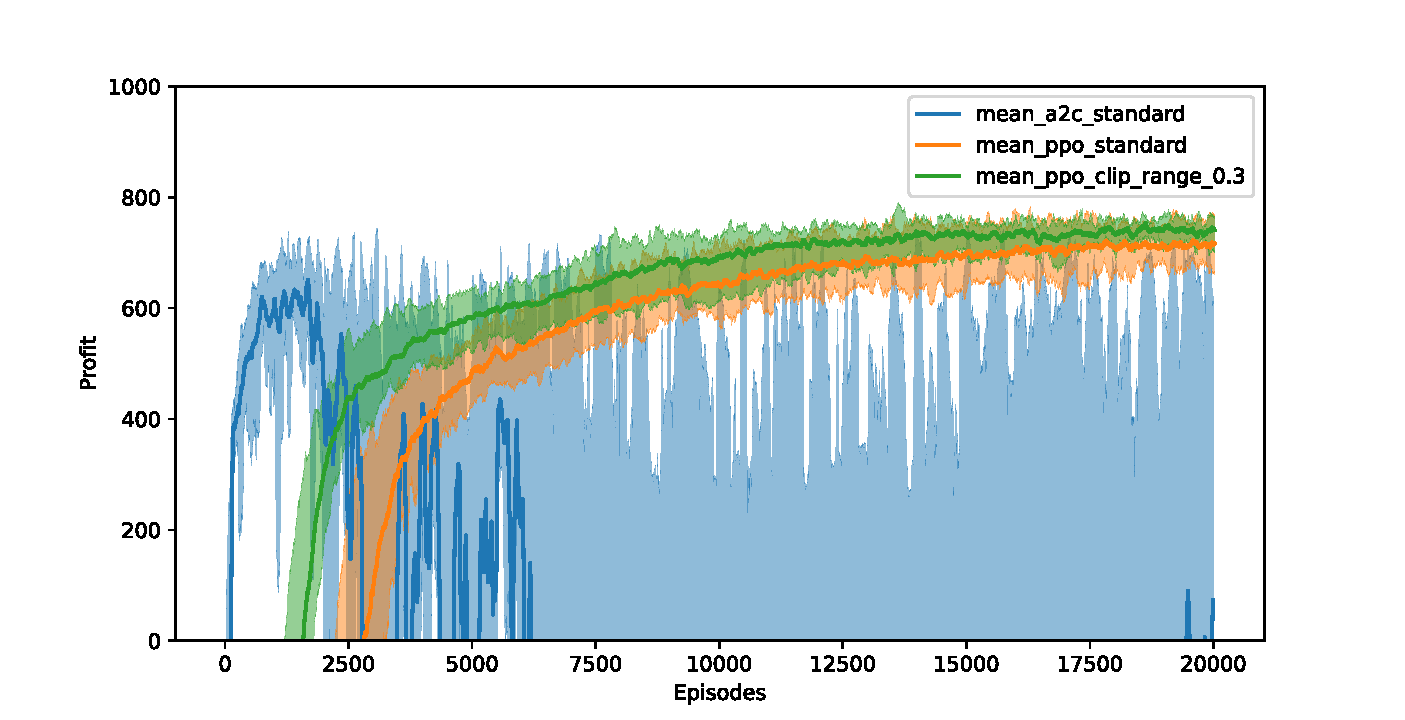
\includegraphics[width=\textwidth]{main/a2c_vs_ppo.pdf}
	\caption{Lernkurven von A2C und PPO auf dem Duopol mit unterbietendem Wettbewerber}
	\label{grafic:OnPolicyLearningCurves}
\end{figure}

Grafik \ref{grafic:OnPolicyLearningCurves} stellt die Lernkurven der Algorithmen dar.
Dabei wurde PPO mit zwei Hyperparametrisierungen verwendet, die sich im Parameter $\epsilon$ unterscheiden.
Das eine Mal wird $0.2$ wie im Originalpaper verwendet, das andere Mal $0.3$.
Jedes dieser Experimente wurde acht Mal unabhängig für eine Million Schritte (zwanzigtausen Episoden) laufen gelassen.
Die Lernkurven verwenden wieder die laufenden Durchschnitte der Episodenreturns.
Der Bereich zwischen maximalem und minimalem Episodenreturns dieser acht Agenten ist eingefärbt.
Die Linie stellt ihren Durchschnitt dar.
In dieser Grafik wird der Verlustbereich ausgeblendet.
Sie stellt nur den Bereich zwischen 0 und 1000 dar, um durch die Skalierung einen genaueren Vergleich im oberen Leistungsbereich zu ermöglichen.

Aus den Grafiken geht unmittelbar hervor, dass alle diese Agenten die Gewinnzone erreichen.
Sie unterscheiden sich in der Spitzenperformance mit Ergebnissen über 500 nicht grundlegend.
Das übertrifft das Durchschnittsergebnis ? des regelbasierten Agenten, wenn er auf diesem Duopolszenario (gegen seine eigene Policy) antritt.
Auf Grundlage dieser Ergebnisse kann man feststellen, dass die Parametrisierung mit $\varepsilon=0.3$ leicht bessere Performance einbringt als die Standardparametrisierung, die wiederung A2C leicht schlägt.
Allerdings erreicht auch A2C in einigen der Spitzen ein sehr hohes Niveau, die Unterschiede zwischen diesen Algorithmen in der Spitzenperformance verschwindend.

Die Advantage-Actor-Critic-Agenten erreichen das hohe Leistungsniveau allerdings nach deutlich weniger Episoden als die PPO-Agenten.
Ihr Durchschnitt überschreitet die Schwelle zum Gewinn nach nur 110 Episoden (umgerechnet 5500 Schritte).
Allerdings ist das Training der A2C-Agenten ausgesprochen instabil.
\begin{figure}[htbp]
	\centering
	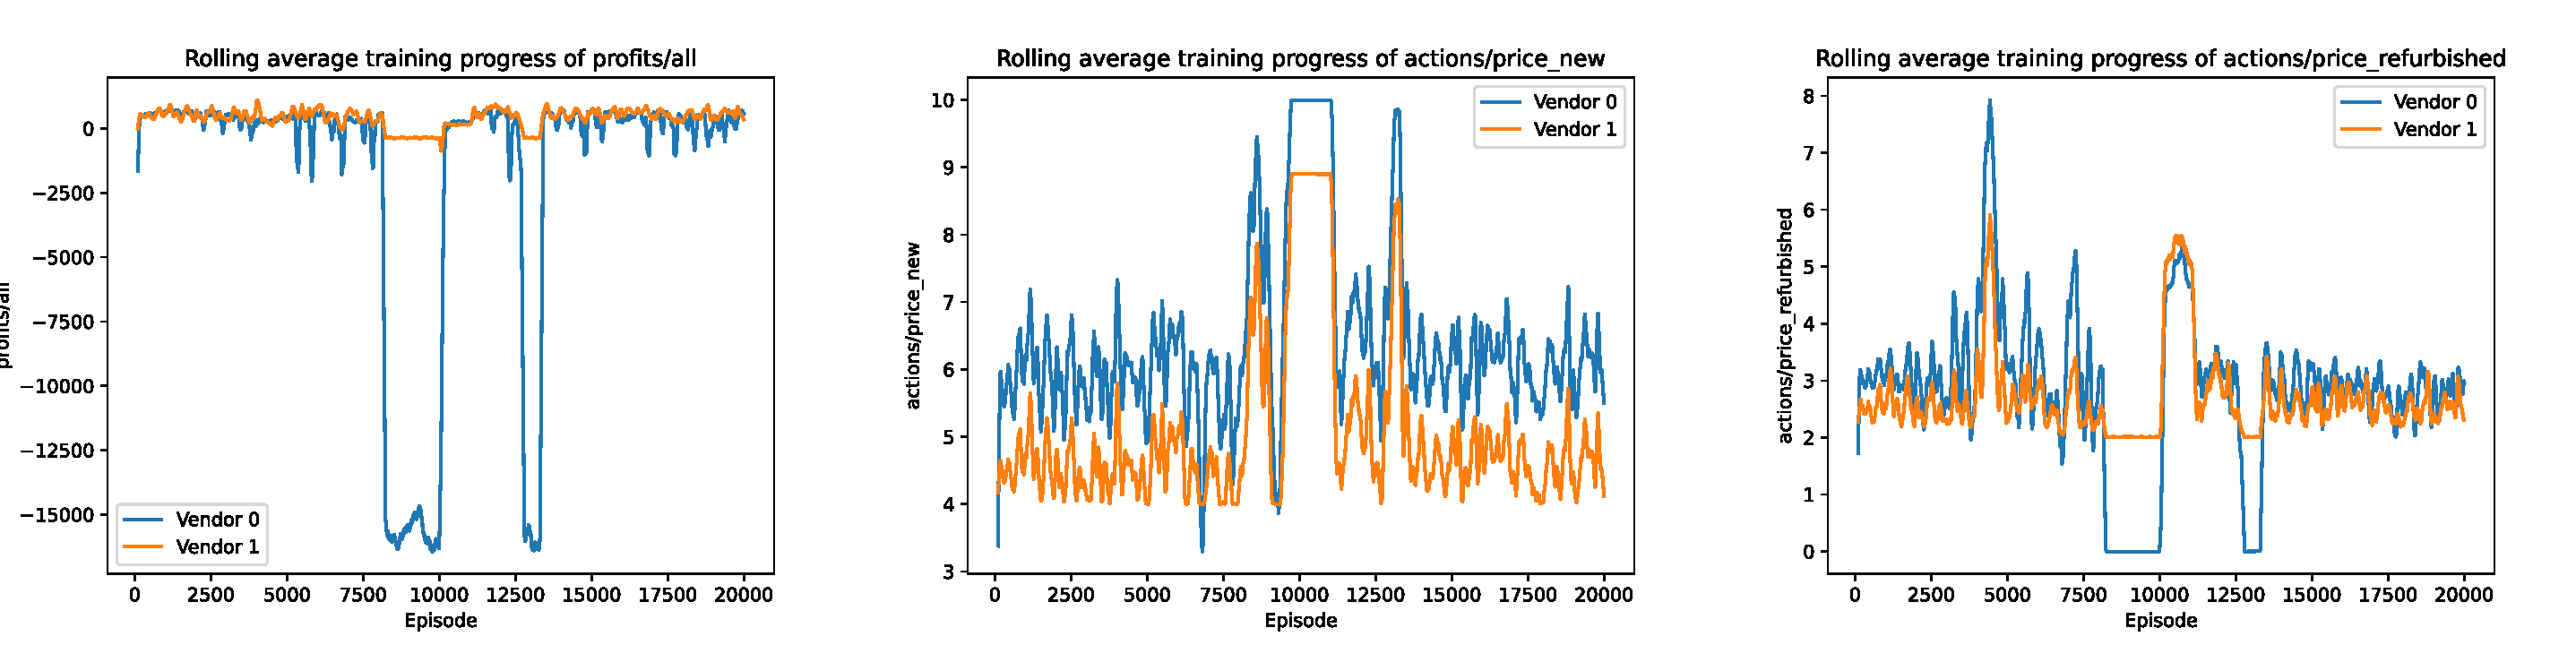
\includegraphics[width=\textwidth]{main/a2c_detailed_analysis.pdf}
	\caption{
		Detaillierte Betrachtung eines A2C-Trainingsdurchlaufes zur Visualisierung der Instabilität, wobei Vendor\_0 der RL-Agent und Vendor\_1 der regelbasierte, direkte Wettbewerber während des Trainings ist:
		(links) Lernkurve mit schnellem initialem Anstieg, danach mehrere Abstürze und Erholungen;
		(mitte) durchschnittliche Auswahl der Neupreise, zeigt erhebliche Schwankungen;
		(rechts) durchschnittliche Auswahl der Gebrauchtpreise, ebenfalls instabil
	}
	\label{grafic:A2CInstability}
\end{figure}
Die Grafik \ref{grafic:A2CInstability} stellt Details eines einzelnen A2C-Durchlaufes dar.
Es handelt sich dabei um einen typischen Durchlauf mit guter Peak-Performance.
Innerhalb der ersten 2000 Episoden erreicht er eine Performance von 748.
Man sieht, dass die Aktionsauswahl während des Trainings permanent hin- und herschwankt.
Wie auch bei den anderen A2C-Agenten stürzt seine Leistung mitunter deutlich ab und fällt dabei weit in die Verlustzone.
Nicht immer erholen sich die Agenten davon, oft erhalten sie weiterhin schlechte Ergebnisse.
Diese heftigen Abstürze führen dazu, dass die Mittelwertlinie der A2C-Agenten in Abbildung \ref{grafic:OnPolicyLearningCurves} wieder unter 0 fällt, obwohl einige der Agenten weiterhin gute Ergebnisse liefern.

Im Gegenzug dazu ist die Trainingsstabilität bei den PPO-Varianten deutlich höher.
Zwischen den acht Trainingsdurchläufen der PPO-Agenten gibt es kaum Unterschiede in der Entwicklung.
Die Leistungsentwicklung liegt in einem schmalen Band und Abstürze finden nicht statt.
Allerdings benötigt PPO in der Standardkonfiguration etwa 2600 Episoden und in der Version mit $0.3$ als $\varepsilon$ ungefähr 1600 Episoden, um die Gewinnzone zu erreichen.
Auch danach ist das Training langsam.
\begin{figure}[htbp]
	\centering
	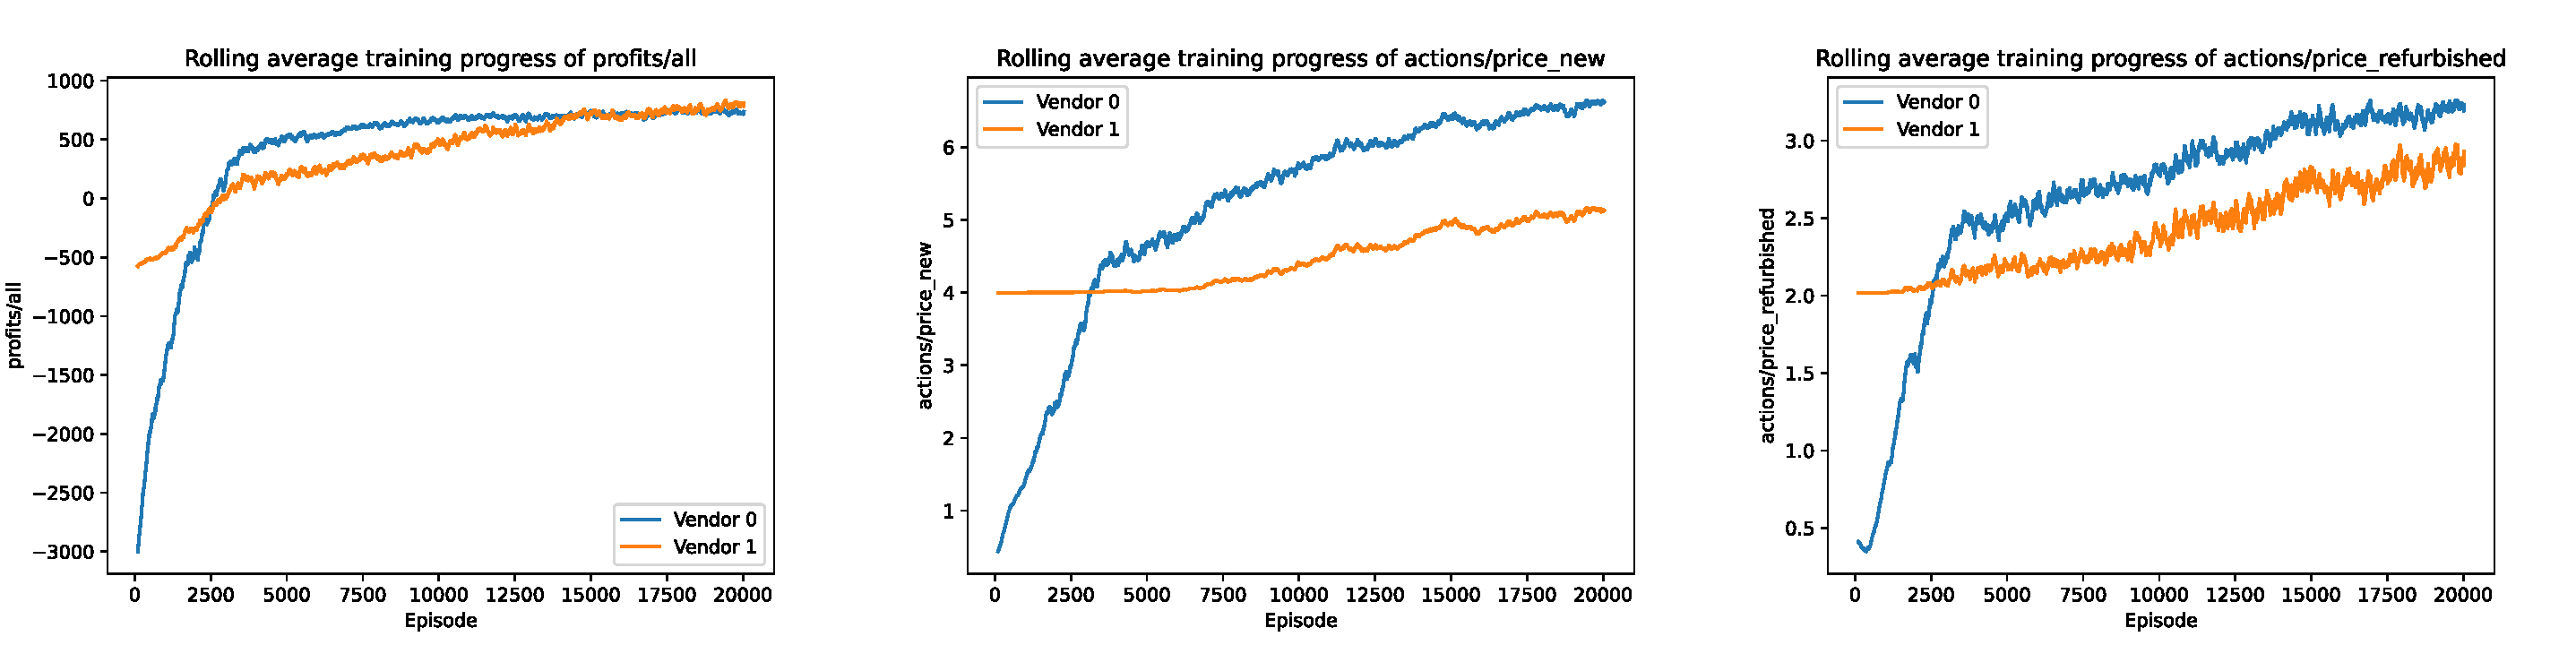
\includegraphics[width=\textwidth]{main/ppo_detailed_analysis.pdf}
	\caption{Detaillierte Betrachtung eines PPO-Trainingsdurchlaufes (Variante mit $\varepsilon=0.2$) analog zu Abbildung \ref{grafic:A2CInstability}}
	\label{grafic:PPOStability}
\end{figure}
In Abbildung \ref{grafic:PPOStability} ist ein detaillierter Blick in einen typischen PPO-Trainingsdurchlauf zu sehen.
Dieser erreicht erst nach etwa 15000 Episoden ein Leistungsniveau von 740, weist aber bei Return und der Aktionsauswahl eine durchweg stabile Entwicklung auf.

Dieser Unterschied von PPO zu A2C überrascht nicht, er existiert \textit{by design}.
Diese Experimente zeigen, dass PPO in seiner Intention, die Trainingsstabilität zu erhöhen, erfolgreich ist.
Diese Erhöhung der Trainingsstabilität findet dadurch statt, dass die Änderung der stochastischen Policy bei den Trainingsschritten begrenzt wird.
Aus dieser Begrenzung der Policyänderung ist die geringere Lerngeschwindigkeit dann eine logische Schlussfolgerung.

So lässt sich auch erklären, warum der Durchlauf mit $\varepsilon=0.3$ schneller trainiert.
Mit größerem $\varepsilon$ wird pro Sample eine größere Policyänderung erlaubt, was zu schnellerem Training führt.
Allerdings steigt damit wieder das Risiko von Instabilität, weshalb die Parametrisierung des PPO-Algorithmus einen Trade-off zwischen Trainingsgeschwindigkeit und Stabilität eröffnet.
Die Wahl des Standardparameters $0.2$ mag in diesen Experimenten konservativ erscheinen, $0.3$ verursacht ebenfalls keine Instabilitäten.
Das Experiment [noch zu erstellen] im Anhang zeigt, wie sich PPO bei größerem $\varepsilon$ verhält.

Eine Beobachtung in Abbildung \ref{grafic:PPOStability} verdient noch einmal besondere Beachtung, weil sie zunächst paradox erscheint:
Obwohl der RL-Agent den regelbasierten Agenten nach etwas Training übertrifft, wird er später wieder wieder überholt.
Das erweckt den Eindruck, als ob der Agent im Verlaufe des Training schlechter würde.
Jedoch ist das Gegenteil der Fall.
Der PPO-Agent erlernt zunächst, die Preise für Neu- und Gebrauchtware höher zu setzen.
Dieses Training dauert aus inzwischen diskutierten Gründen relativ lange, aber bei Neuverkaufspreisen, die größer als vier sind, macht er die Erfahrung, dass der regelbasierte Wettbewerber ihn immer um 1 unterbietet.
Durch wechselseitiges Unterbieten führt eine Preisabwärtsspirale dazu, dass sich der Preis nur knapp überhalb des Einkaufspreises einpegelt.
Die dabei äußerst niedrige Rendite ermöglicht jedoch nur niedrige Gewinne, sodass der Agent in seinem weiteren Training die Erfahrung macht, dass er seinen Gewinn steigern kann, indem er seine Preise höher setzt.
Er wird dann zwar immer noch unterboten, allerdings nur um den Wert eins.
Dabei nimmt er in Kauf, dass mehr Kunden wegen des niedrigen Preises beim Konkurrenten kaufen und dieser auch an jedem Kunden noch mehr verdient.
Mit den Kunden, die der RL-Agent aber noch bekommt, kann er aber seine Gewinne im Vergleich zum niedrigpreisigen Markt dennoch steigern.
Der Effekt besteht also darin, dass der RL-Agent in Reaktion auf den ihn immer unterbietenden Konkurrenten diesem einen überproportionalen Gewinnanstieg erlaubt, um selbst mehr Gewinne machen zu können.
Dass sich dieser Effekt so wiederfindet, ist der Tatsache geschuldet, dass das einzige Optimierungskriterium für die Agenten der eigene Gewinn ist.
Eine Rewardformulierung, die ein Übertreffen des Konkurrenten mit einbezieht, wird in Abschnitt [wenn es noch im Scope ist] behandelt.

\section{Soft Actor Critic}
\label{section:main_sac}
Das in Abschnitt \ref{section:sac} erläuternte Soft-Actor-Critic-Verfahren ist in erster Linie für stetige Aktionsräume entwickelt worden und wird hier auch in der stetigen Variante genutzt.
Beim Verfahren wurden die gängigen Hyperparameter eingesetzt.
Die Übersicht dazu findet sich im Anhang in Tabelle ?.
Bei den hier gezeigten Ergebnissen wurde der Entropiekoeffizient $\alpha$ automatisch trainiert.
Er hat sich bei allen Trainingsdurchläufen zwischen $1$ und $1.5$ eingependelt.
Die Grafik ? im Anhang zeigt, dass unterschiedliche manuell eingestellte Entropiekoeffizienten ähnliche Trainingsergebnisse erreichen, wobei sich die Vermutung bestätigt, dass sehr niedrige Entropiekoeffizienten zu wenig Exploration bezwecken und Läufe mit deutlich höheren Entropiekoeffizienten bei schlechterer Leistung verharren.

\begin{figure}[htbp]
	\centering
	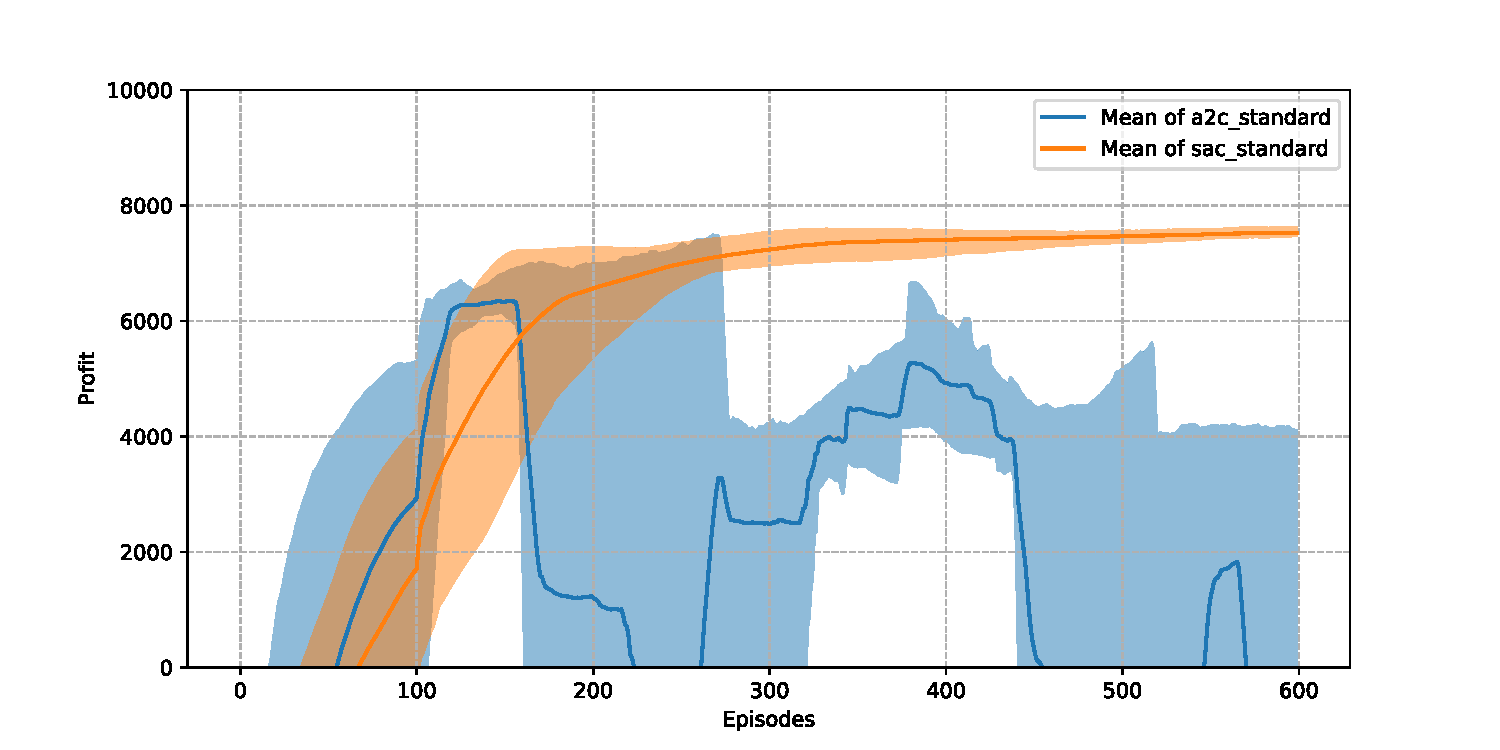
\includegraphics[width=\textwidth]{main/a2c_vs_sac.pdf}
	\caption{Lernkurve von Soft Actor Critic über 4000 Episoden, A2C als Vergleich angegeben}
	\label{grafic:SACLearningCurve}
\end{figure}

Grafik \ref{grafic:SACLearningCurve} zeigt die Lernkurve von acht Soft-Actor-Critic-Agenten bei einem Trainingsdurchlauf mit 4000 Episoden (200000 Schritte).
Zum Vergleich sind acht Trainingsdurchläufe mit A2C angegeben, die den aus Abschnitt \ref{section:main_ppo} bekannten Verlauf aufweisen.
Soft-Actor-Critic wurde als Off-Policy-Algorithmus neben dem Erreichen von wettbewerbsfähigen Ergebnissen für zwei Hauptziele entwickelt:
Erstens soll es eine sehr hohe Sample Efficiency haben, was bedeutet, dass es beim Training deutlich weniger Schritten benötigt.
Zweitens soll SAC eine sehr hohe Trainingsstabilität haben.
Die Lernkurve bestätigt, dass Soft-Actor-Critic diese zwei Hauptziele erreicht.
Profitabel arbeitet der Agent nach etwa 300 Episoden, was etwa auf dem Level von A2C liegt und erheblich besser als PPO ist.
Spitzenperformance wird ähnlich wie bei A2C nach 500 bis 1000 Episoden erreicht.
Der weitere Trainingsverlauf ist sehr stabil.
Alle acht Agenten bewegen sich für den Rest des Trainings in einem sehr schmalen Bereich, wobei der Durchschnittsreturn der Agenten bei etwa 660 konstant bleibt.
Eine Verbesserung der Leistung findet nach etwa 1500 Episoden nicht mehr statt und auch die Spitzenwerte einiger der SAC-Agenten werden ab dort nicht wieder erreicht.
Der Durchschnitt der acht SAC-Agenten liegt zwar dauerhaft über dem Durchschnitt der A2C-Agenten, aber einige A2C-Durchläufe übertreffen in ihren Spitzenwerten alle SAC-Agenten.
Mit der Spitzenperformance der PPO-Agenten kann SAC ebenfalls nicht ganz mithalten.

\begin{figure}[htbp]
	\centering
	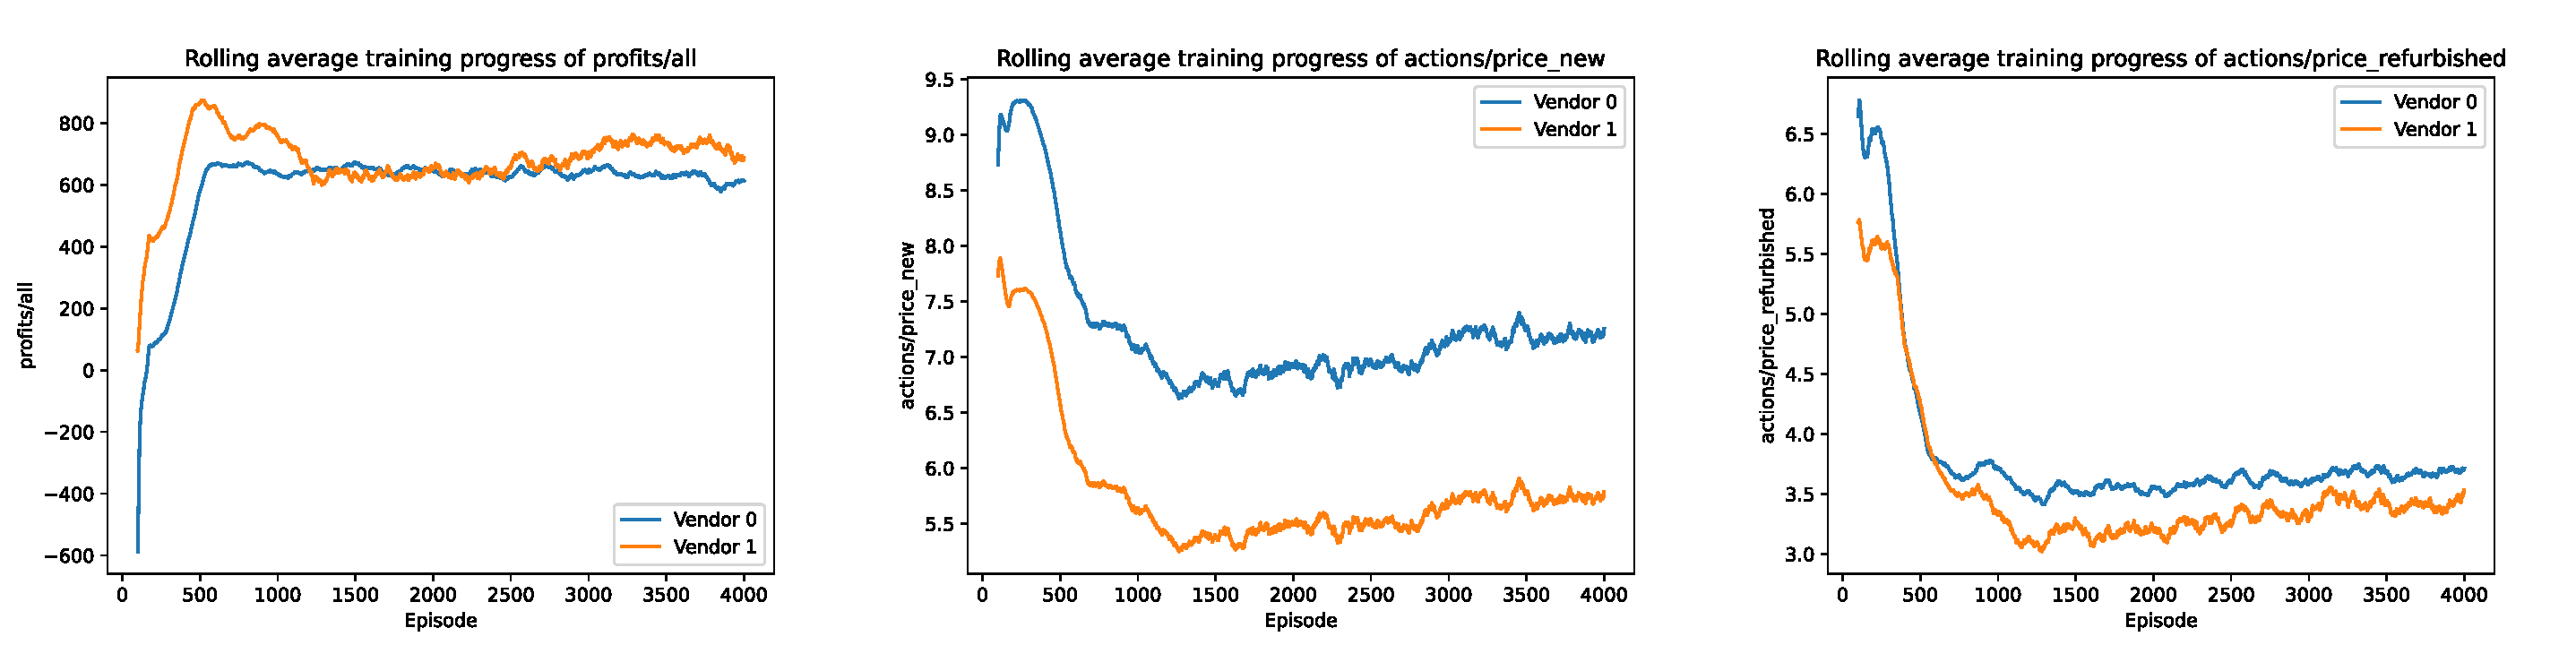
\includegraphics[width=\textwidth]{main/sac_detailed_analysis.pdf}
	\caption{Detaillierte Betrachtung eines SAC-Trainingsdurchlaufes}
	\label{grafic:SACDetails}
\end{figure}

Wie auch für die anderen Algorithmen wurde für SAC ein typischer Durchlauf und die gemittelten Aktionen in Abbildung \ref{grafic:SACDetails} abgedruckt.
Dieser ist stabil und weist abgesehen vom Start mit höheren Werten ein ähnliches Profil wie der PPO-Durchlauf auf:
Zunächst sinken die Preise auf ein niedriges Niveau und steigen dann leicht an.
Während die Gebrauchtpreise zwischen diesem SAC- und dem PPO-Durchlauf sehr ähnlich sind, liegen die Neupreise hier auf etwas höherem Niveau.

Für die Frage >>Wie lange dauert das Training?<< gibt es zwei mögliche Kenngrößen.
Einmal können die benötigten Samples herangezogen werden, die Sample Efficiency, oder es kann die tatsächliche Zeit auf der Uhr bewertet werden.
Letztere hängt stark von der Hardware sowie der Geschwindigkeit der Simulation im Vergleich zum Optimieren der Parameter ab.
Bei der für diese Experimente verwendeten Implementierung und Hardware benötigt das Training pro Schritt mit SAC etwa $3.7$ Mal so lang wie mit PPO.
Das Sammeln der Beispiele aus dem Markt nimmt bei PPO etwa 25\% der Trainingszeit ein, bei SAC nur etwa 6\%.
Die Geschwindigkeiten von A2C sind denen von PPO sehr ähnlich.
Rechnet man somit die tatsächliche Trainingszeit, relativiert sich der höhere Samplebedarf bei PPO.
Er erreicht die Gewinnzone nur etwa 50\% später als SAC.
Dabei wird klar, dass A2C in reinem Zeitbedarf den anderen Algorithmen deutlich überlegen ist.

\section{Training gegen die eigene Policy}
Die in den Abschnitten \ref{section:main_ddpg}, \ref{section:main_ppo} und \ref{section:main_sac} betrachteten Durchläufe trainierten die RL-Agenten alle gegen den in Abschnitt \ref{section:rulebased} definierten regelbasierten Wettbewerber.
Das erfüllt die theoretischen Anforderungen eines Markov-Entscheidungsprozesses, stellt jedoch für praktische Anwendungen eine Reihe von Problemen auf.
Erstens muss dafür die Policy des Konkurrenten bekannt sein.
Weil jedoch davon ausgegangen werden kann, dass der Konkurrent seine Preisstrategie nicht verraten wird, müsste sie unter Inkaufnahme von Ungenauigkeiten aus historischen Daten geschätzt werden.
Zweitens ist die mittels RL trainierte Strategie nur gegen diese bestimmte regelbasierte Strategie gerichtet.
Ändert der Wettbewerber seine Preisstrategie plötzlich, schwächt das die Performance der RL-Strategie und macht neues Training erforderlich.
Um jedoch die neue Strategie für das erneute RL-Training verstehen zu können, werden wieder historische Daten benötigt, die zunächst nicht vorliegen.

Deshalb wünscht man sich eine Strategie, die gegen möglichst viele Wettbewerberstrategien bestehen kann, nicht auf eine spezielle overfittet ist.
Deepmind hatte eine ähnliche Herausforderung beim Training von Go- und Schachstrategien, das sie durch Self-Play gelöst haben. \cite{Silver2017, https://doi.org/10.48550/arxiv.1712.01815}
Für diesen Markt wurde eine Self-Play Variante entwickelt, bei der ein RL-Agent weiterhin auf einem Duopol-Markt trainiert, aber die Policy des Wettbewerbers die eigene Policy ist.
In der programmiertechnischen Umsetzung wird dann für den Gegner ein Zeiger auf den RL-Agenten übergeben, der schließlich auch die Policyfunktion implementiert.
Dadurch, dass der Agent stets gegen sich selbst spielt, wird die Markov-Eigenschaft verletzt, dennoch zeigen die Ergebnisse Trainingserfolg.
Die Motivation hinter Self-Play ist, dass der Agent einerseits stets einem ebenbürtigen Gegner gegenübersteht, aber andererseits auch, dass er ständig Strategien gegen die eigene entwickelt, die dann wiederum herausgefordert werden.
Dadurch soll der Agent gegen eine Vielzahl von Policies gestählert werden.
Experimente mit Self-Play wurden mit den Algorithmen durchgeführt, die sich in der vorangegangenen Analyse als grundsätzlich geeignet für diesen Markt erwiesen haben: A2C, PPO und SAC.

\begin{figure}[htbp]
	\centering
	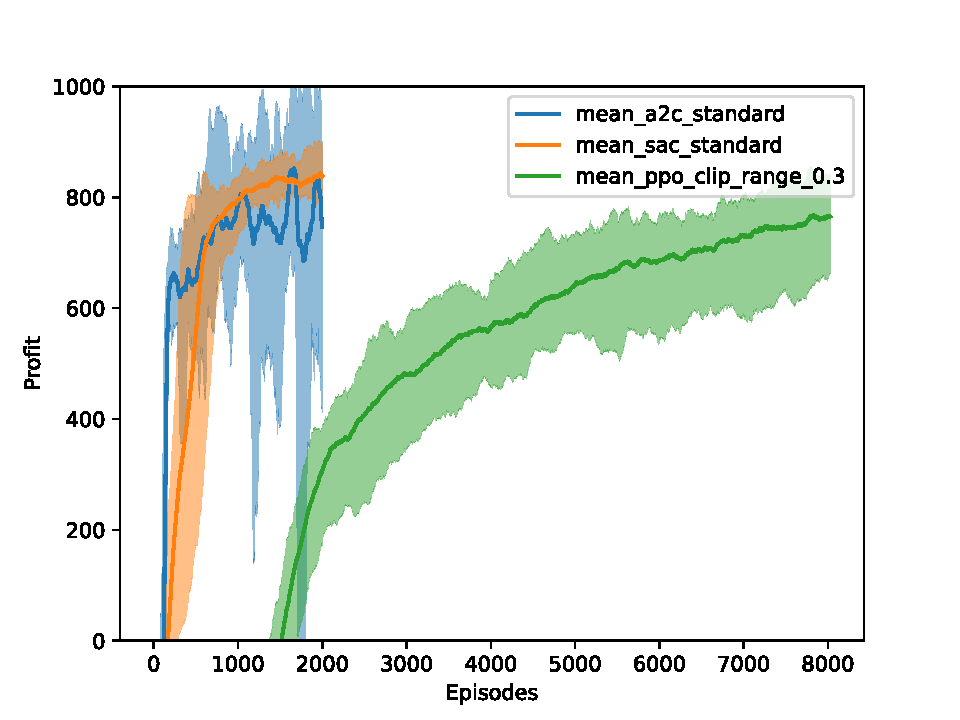
\includegraphics[width=\textwidth]{main/self_play.pdf}
	\caption{Lernkurve von A2C, PPO und SAC beim Self-Play; A2C und SAC wurden über 2000 Episoden trainiert, PPO über 8000}
	\label{grafic:SelfPlayLearningCurve}
\end{figure}
In der Abbildung \ref{grafic:SelfPlayLearningCurve} sind die Lernkurven der drei Algorithmen beim Training gegen sich selbst abgedruckt.
Diese Kurven zeigen zunächst, dass Lernerfolg bei allen dieser drei Agenten erreicht wird.
Sie sind aber alleine nicht aussagekräftig, ob die Agenten sich tatsächlich gegen die Konkurrenz behaupten können.
Deshalb dürfen auch die Returns dieser Lernkurven nicht mit den aus den vorigen Abschnitten verglichen werden.

\begin{figure}[htbp]
	\centering
	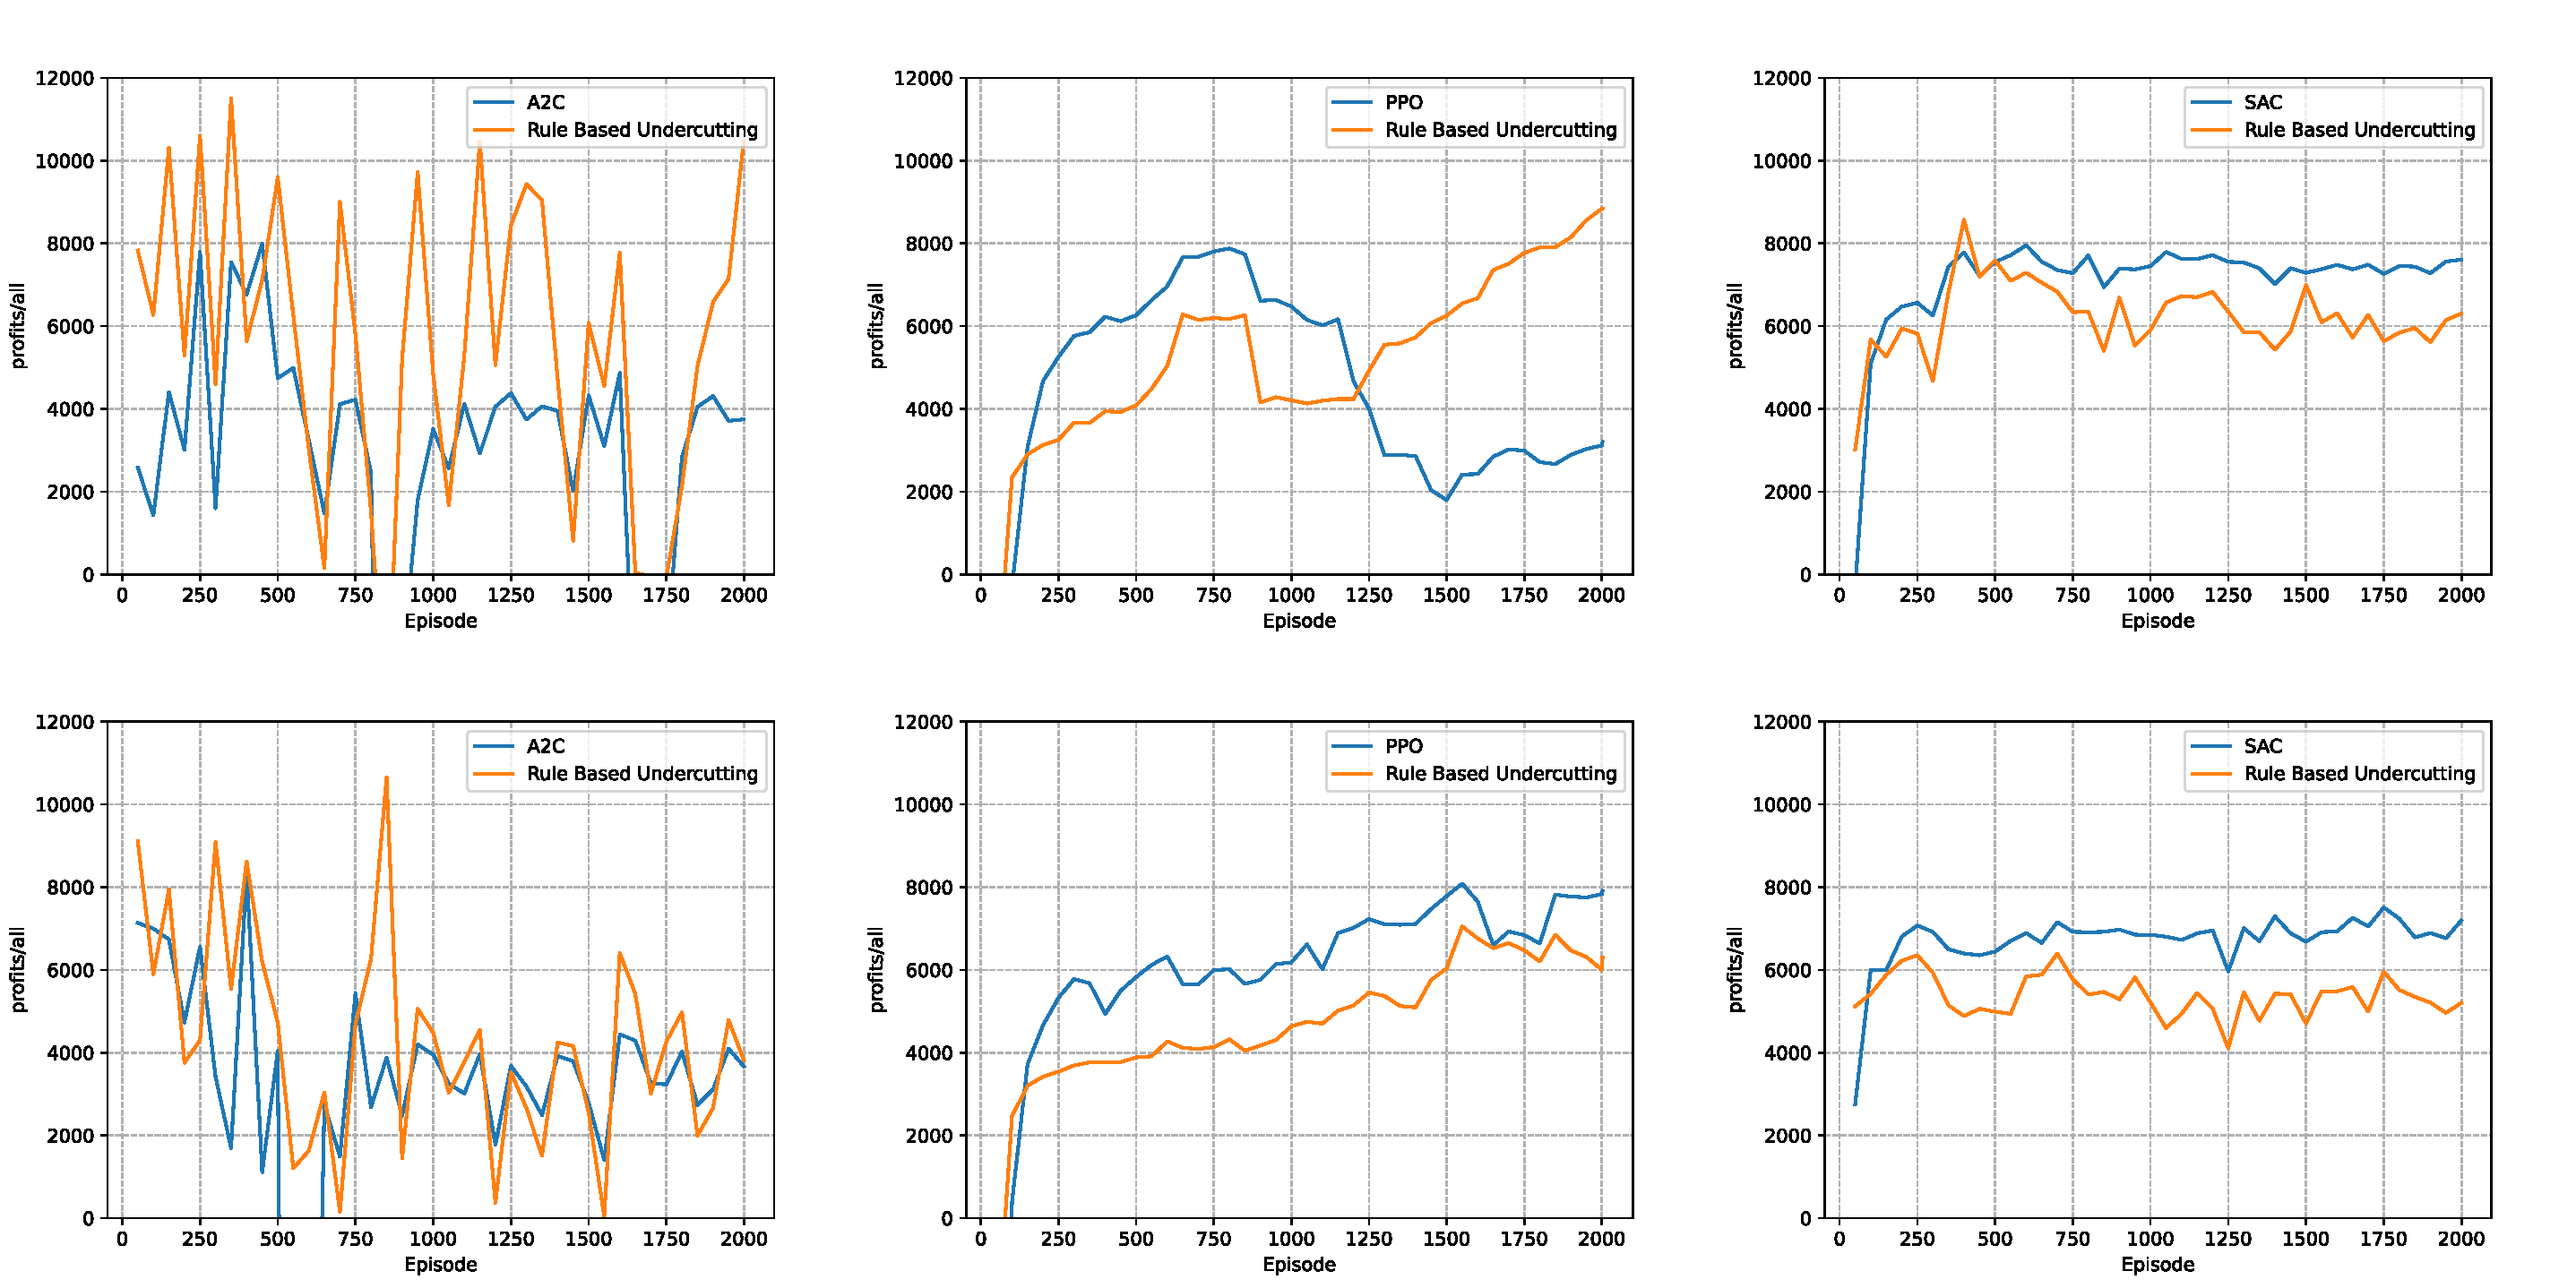
\includegraphics[width=0.8\textwidth]{main/self_play_detailed.pdf}
	\caption{
        Einzelne Self-Play-Trainingsdurchläufe der Algorithmen:
        (links) Trainingsverlauf im Vergleich zum regelbasierten Agenten;
        (rechts) Verteilung der Gewinne des RL-Agenten im Vergleich zum regelbasierten an der Stelle mit maximaler Belohnung
    }
	\label{grafic:SelfPlayDetails}
\end{figure}
Um Vergleichbarkeit herstellen zu können, wurde während des Self-Plays alle 100 Episoden ein Modell gespeichert und jedes dieser Modelle anschließend auf 250 Episoden getestet.
Damit wurden Verteilungen und Kenngrößen gemessen, um eine akurate Lernkurve erstellen zu können, die das beim Self-Play trainierte Modell mit dem regelbasierten Agenten vergleicht.
Von allen Algorithmen wurde ein mittlerer Durchlauf ausgewählt und in der Abbildung \ref{grafic:SelfPlayDetails} veranschaulicht.
Dabei stellt sich heraus, dass die Agenten den Markt erfolgreich erlernt haben.
Die Maxima dieser mittleren Durchläufe liegen bei 745 (A2C), 545 (PPO) und 630 (SAC).
Das ist über dem Niveau, das der regelbasierte Wettbewerber gegen sich selbst erreicht, und reicht erwartungsgemäß nicht ganz an die Ergebnisse des Trainings direkt gegen den regelbasierten Agenten heran.
Auch wenn das nicht explizites Trainingsziel war, übertreffen die Agenten dennoch die regelbasierte Konkurrenz.
Bemerkenswert an diesen Ergebnissen ist jedoch, dass sie erreicht wurden, ohne den regelbasierten Wettbewerber je vorher gesehen zu haben.
Die Lernkurven lassen zudem vermuten, dass bei PPO eine weitere Steigerung der Leistung möglich ist.\footnote{Wenn ich hier noch länger gewartet hätte, hätte ich den Draft nicht mehr fertig bekommen}
